\documentclass[12pt,a4paper]{article}

\usepackage[utf8]{inputenc}
\usepackage[T1]{fontenc}
\usepackage{polski}

\usepackage{amsthm}
\usepackage{amsmath}
\usepackage{amsfonts}
\usepackage{amssymb}
\usepackage{pgfplots}
\usepackage{tikz}
\usepackage{lmodern}	%fancy font
\usepackage{textcomp}

\usepackage{indentfirst}
\usepackage{graphicx}
\usepackage{caption}
\usepackage{subcaption}
\usepackage{siunitx}
\usepackage{here}


\setlength{\textheight}{24cm}
\setlength{\textwidth}{15.92cm}
\setlength{\footskip}{10mm}
\setlength{\oddsidemargin}{0mm}
\setlength{\evensidemargin}{0mm}
\setlength{\topmargin}{0mm}
\setlength{\headsep}{5mm}
\usepackage{tikz}
\usepackage{lmodern}	%fancy font
\usepackage{textcomp}

\usepackage{indentfirst}
\usepackage{graphicx}
\usepackage{caption}
\usepackage{subcaption}
\usepackage{siunitx}
\usepackage{here}
\usepackage[margin=1in]{geometry}% Just for this example
\setlength{\parindent}{0pt}% Just for this example
\setlength{\textheight}{24cm}
\setlength{\textwidth}{15.92cm}
\setlength{\footskip}{10mm}
\setlength{\oddsidemargin}{0mm}
\setlength{\evensidemargin}{0mm}
\setlength{\topmargin}{0mm}


\begin{document}

\begin{table}[]
\label{my-label}
\begin{tabular}{|p{7.5cm}|p{7.5cm}|}
\hline
									           					&                           \\

\includegraphics[height=3cm]{logo}             					& \textbf{Technika cyfrowa} \\ \hline
\multicolumn{1}{|l|}{\textbf{Temat ćwiczenia}} 					& \textbf{Numer ćwiczenia}  \\
\multicolumn{1}{|l|}{Bramki logiczne i proste funkcje logiczne}	& 1                         \\ \hline
\multicolumn{1}{|l|}{\textbf{Wykonawca}}       & \textbf{Ocena}            \\
\multicolumn{1}{|l|}{Miron Markowski}          &                           \\ \hline
\end{tabular}
\end{table}

\section{Cel ćwiczenia}

Zapoznanie się z podstawowymi bramkami logicznymi i funkcjami logicznymi oraz skonstruowanie tablic prawdy dla bramek AND, OR, NOR, NAND, XOR, XNOR.



\section{Przebieg ćwiczenia}

\subsection{Tabele prawdy}
W programie multisim przetestowałem podane bramki logiczne:

\begin{center}
\includegraphics[width=.7\textwidth]{tabela}
\end{center}

\begin{table}[H]
\begin{center}

\label{logiczne}
\begin{tabular}{|p{1.1cm}|p{1.1cm}|p{1.1cm}|p{1.1cm}|p{1.1cm}|p{1.1cm}|p{1.1cm}|p{1.1cm}|}
\hline
p & q & AND & OR & XOR & NAND & NOR & XNOR \\ \hline
0 & 0 & 0 & 0 & 0 & 1 & 1 & 1 \\ \hline
0 & 1 & 0 & 1 & 1 & 1 & 0 & 0 \\ \hline
1 & 0 & 0 & 1 & 1 & 1 & 0 & 0 \\ \hline
1 & 1 & 1 & 1 & 0 & 0 & 0 & 1 \\ \hline
\end{tabular}
\caption{Tabela prawdy dla podanych bramek logicznych}
\end{center}
\end{table}

\subsection{Pięciowejściowa bramka AND}
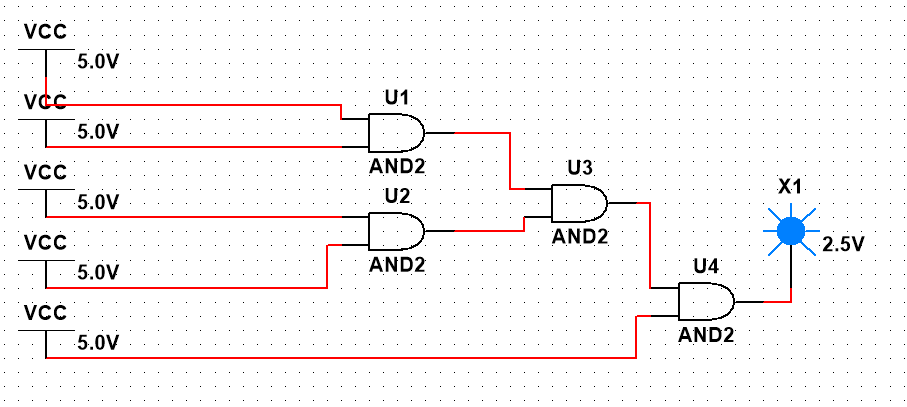
\includegraphics[width=\textwidth]{AND5}
Aby zbudować pięciowejściową bramkę AND potrzeba 4 zwykłych dwuwejściowych bramek. Każde z wejść musi być w stanie wysokim, aby na wyjściu również był stan wysoki.

\subsection{Czterowejściowa bramka OR}
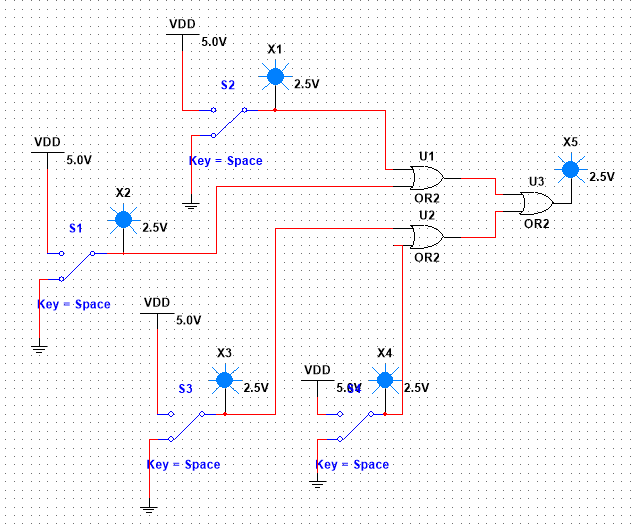
\includegraphics[width=.9\textwidth]{OR4}
Zaobserwowałem, że gdy dowolne wejście jest w stanie wysokim, wyjście również przyjmuje stan wysoki. 

\subsection{Trzywejściowa bramka NAND}
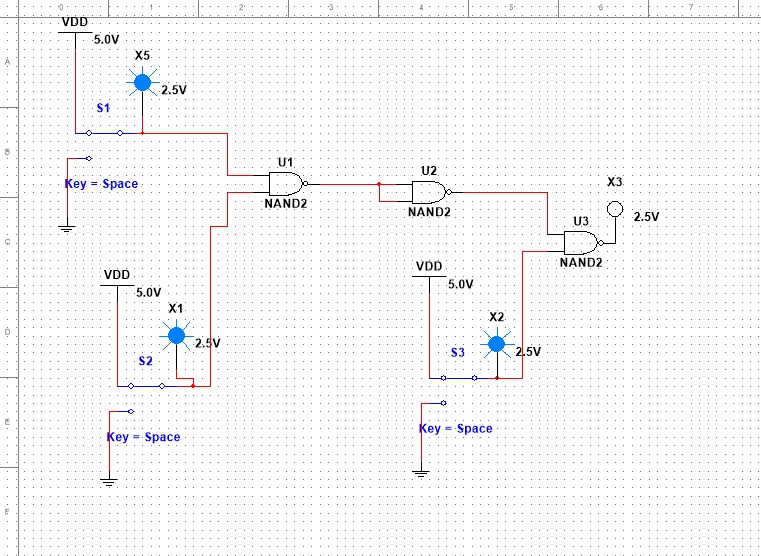
\includegraphics[width=\textwidth]{NAND3}
Ta bramka na wyjściu daje stan wysoki tylko jeśli każde z wejść jest w stanie niskim.

\subsection{Przekształcenia na bramki NOR i NAND}
Tutaj wstaw własnoręcznie zrobione przekształcenia
\newpage
Y = not A\\
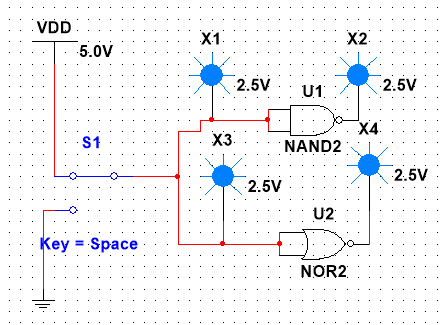
\includegraphics[width=\textwidth]{1e1}
Y = not A and B\\
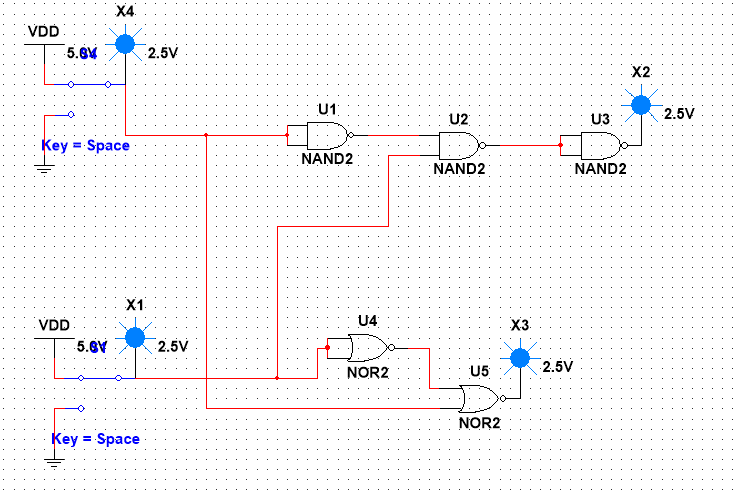
\includegraphics[width=\textwidth]{1e2}
\newpage
Y = A or B\\
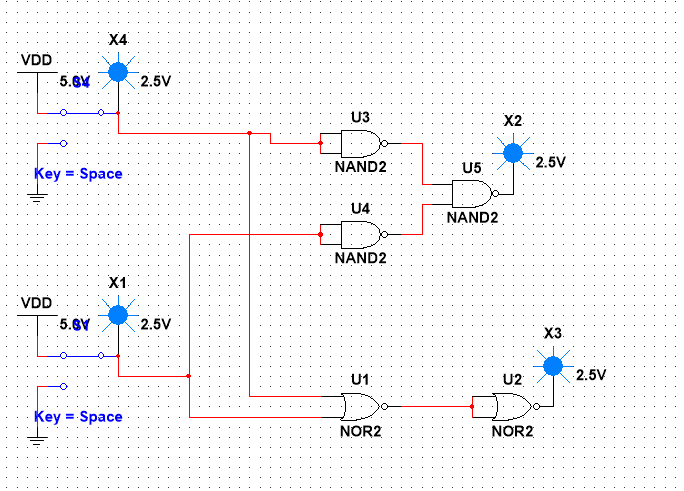
\includegraphics[width=\textwidth]{1e3}
Y = A XOR B\\
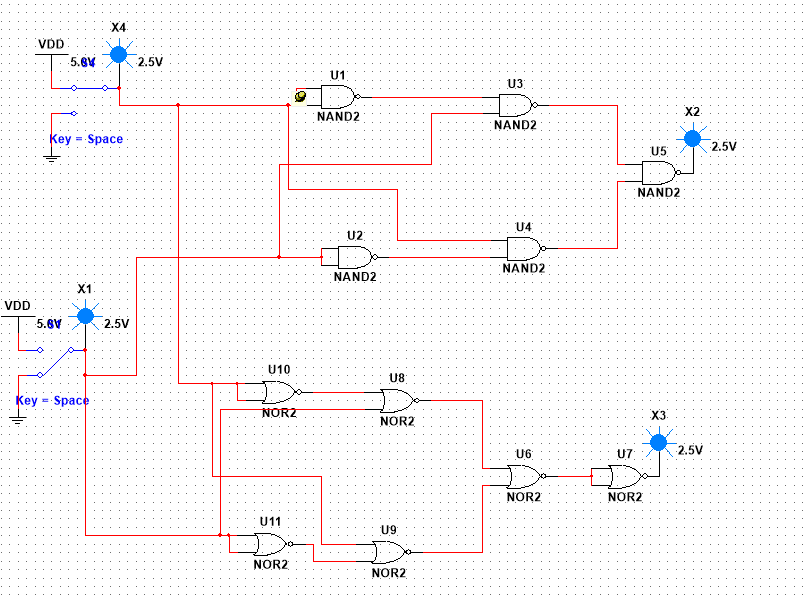
\includegraphics[width=\textwidth]{1e4}



\end{document}